% !TEX root = ../../main.tex

% --------------------------------------
% labels: \label{mil2:res:[type]:[name]}
% --------------------------------------
% PAST TENSE

The free electron fraction as computed from the Saha and Peebles equations in their respective regimes is plotted in~\cref{mil2:res:fig:electron_fraction}. We added the result from using only the Saha equation.
\begin{figure}[!ht]
    \centering
    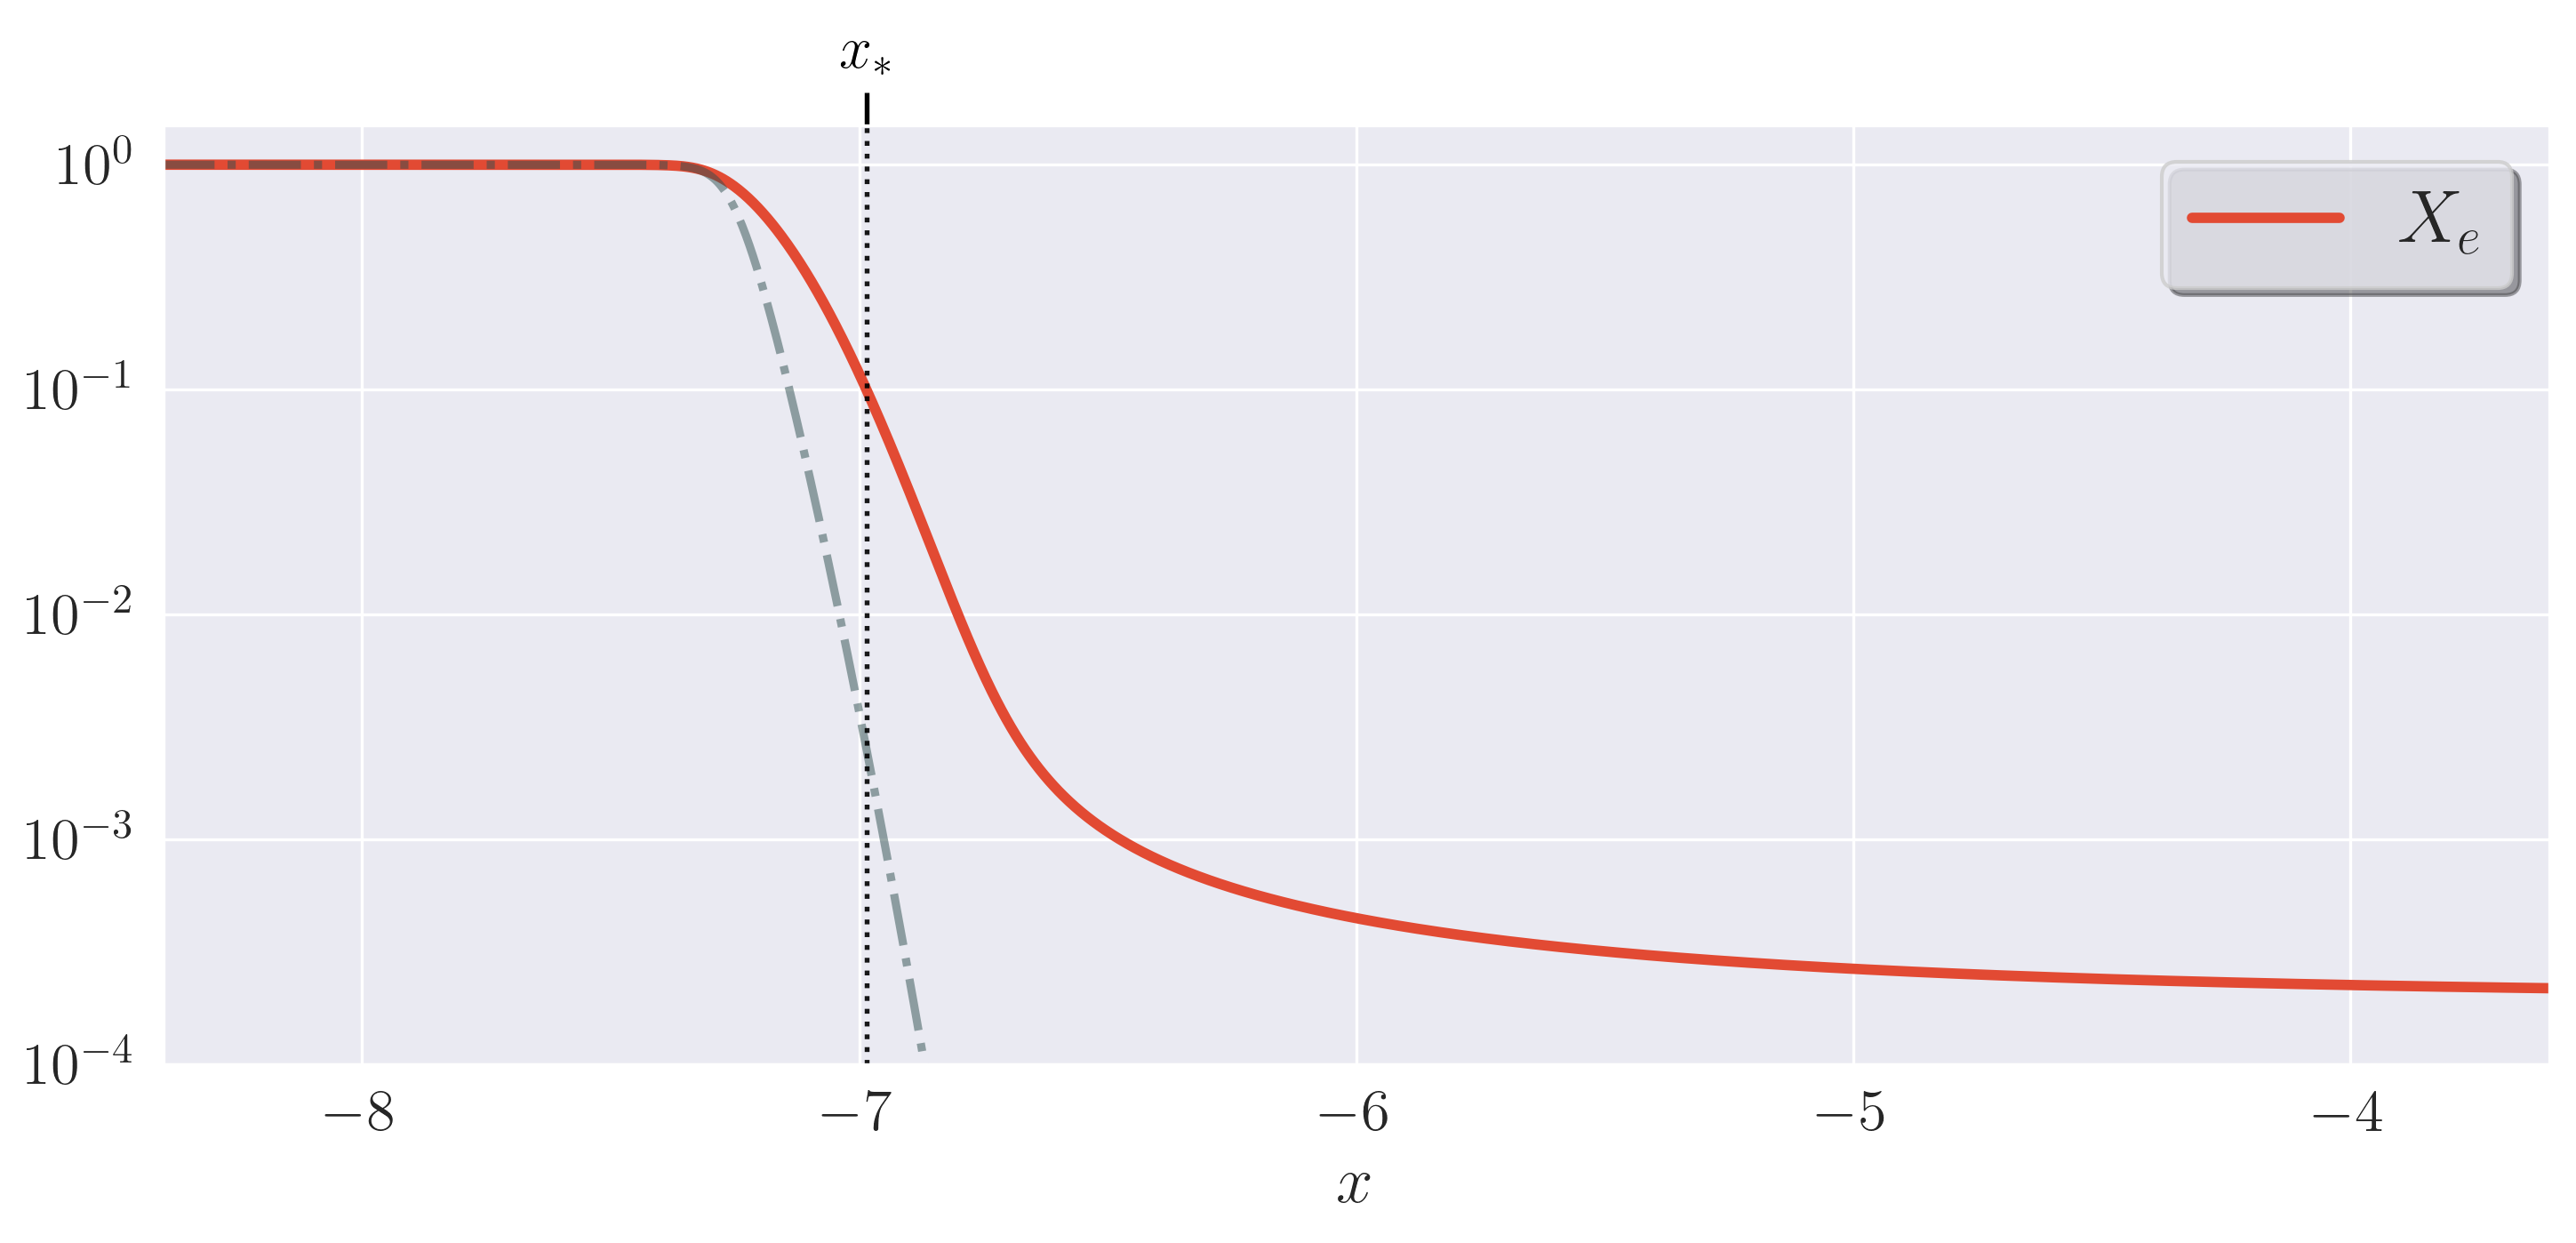
\includegraphics[width=\linewidth]{milestone2/electron_fraction.png} 
    \caption{The free electron fraction $X_e(x)$ resulting from the Saha and Peebles equations. The dash-dotted line represents the solution from the Saha equation only. Recombination onset is shown as the black, dotted vertical line. The freeze-out abundance $X_e\ap{(fo)}= X_e(0)$ is demonstrated as a dotted horizontal line.} 
    \label[fig]{mil2:res:fig:electron_fraction}
\end{figure}
As elaborated in~\cref{mil2:sec:imp} we calculated the optical depth and visibility function and their derivatives.
We present the optical depth and its derivatives in~\cref{mil2:res:fig:optical_depth}. The visibility function is demonstrated in~\cref{mil2:res:fig:visibility_function}, where we have included its derivatives scaled to be comparable to the original function.
\begin{figure}[!ht]
    \centering
    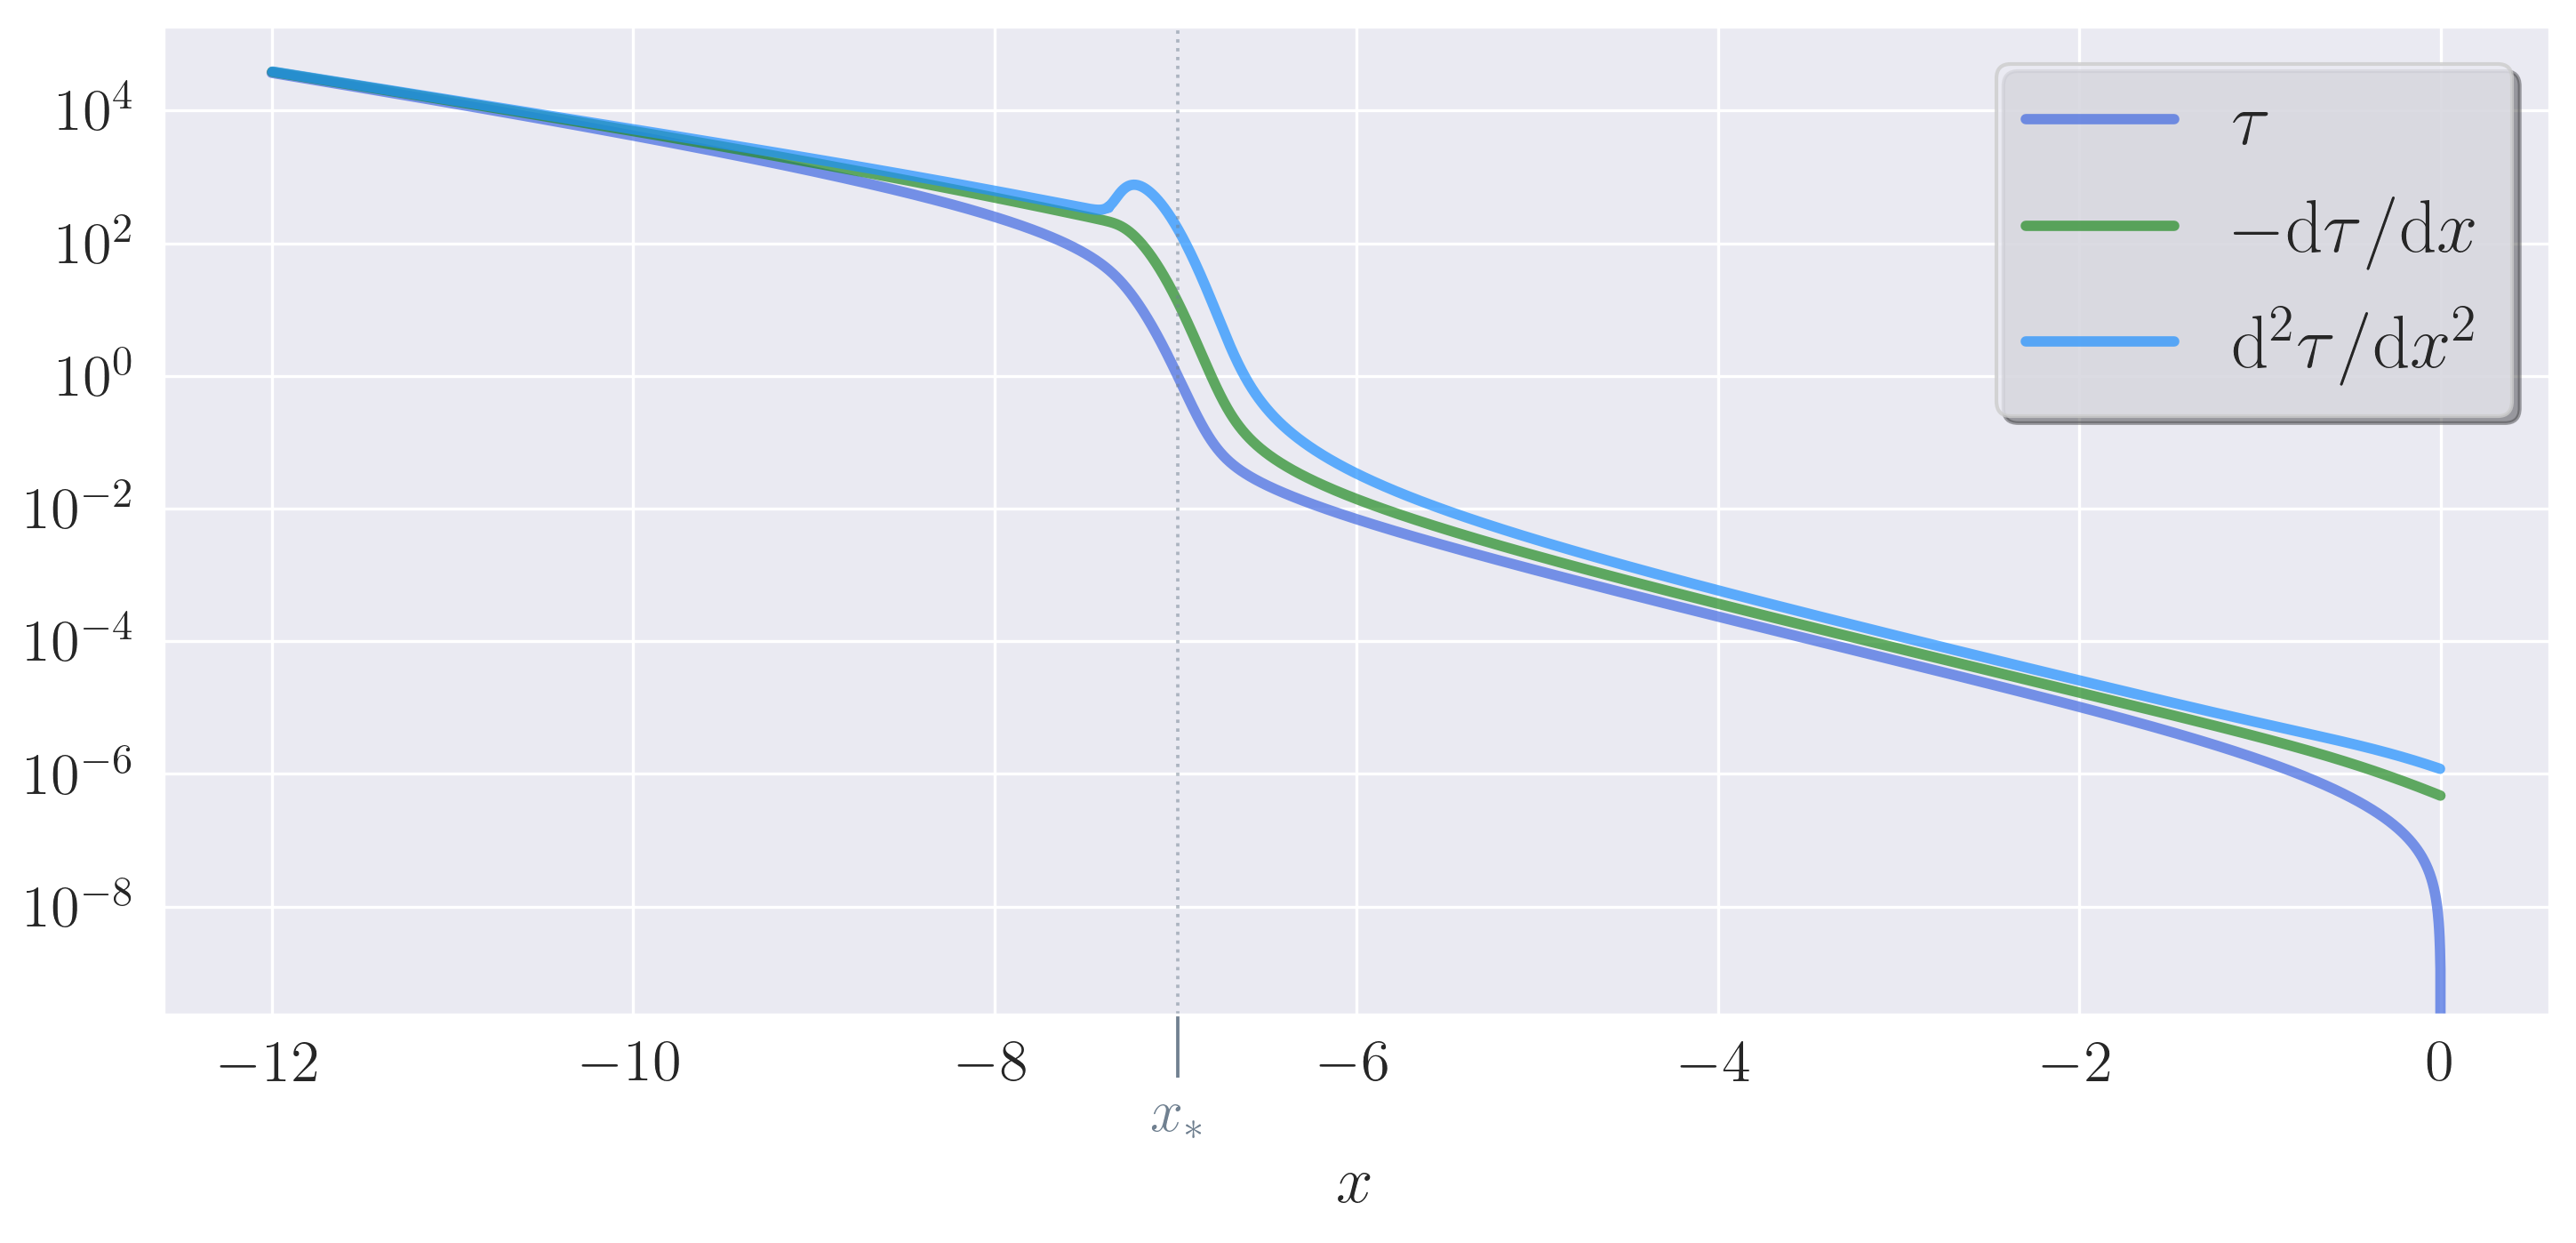
\includegraphics[width=\linewidth]{milestone2/optical_depth_misc.png} 
    \caption{The optical depth $\tau(x)$ and its derivatives $-\dv{\tau(x)}{x}$ and $\dv[2]{\tau(x)}{x}$ as functions of logarithmic scale factor $x$. Recombination onset is shown as the dotted vertical line.} 
    \label[fig]{mil2:res:fig:optical_depth}
\end{figure}
\begin{figure}[!ht]
    \centering
    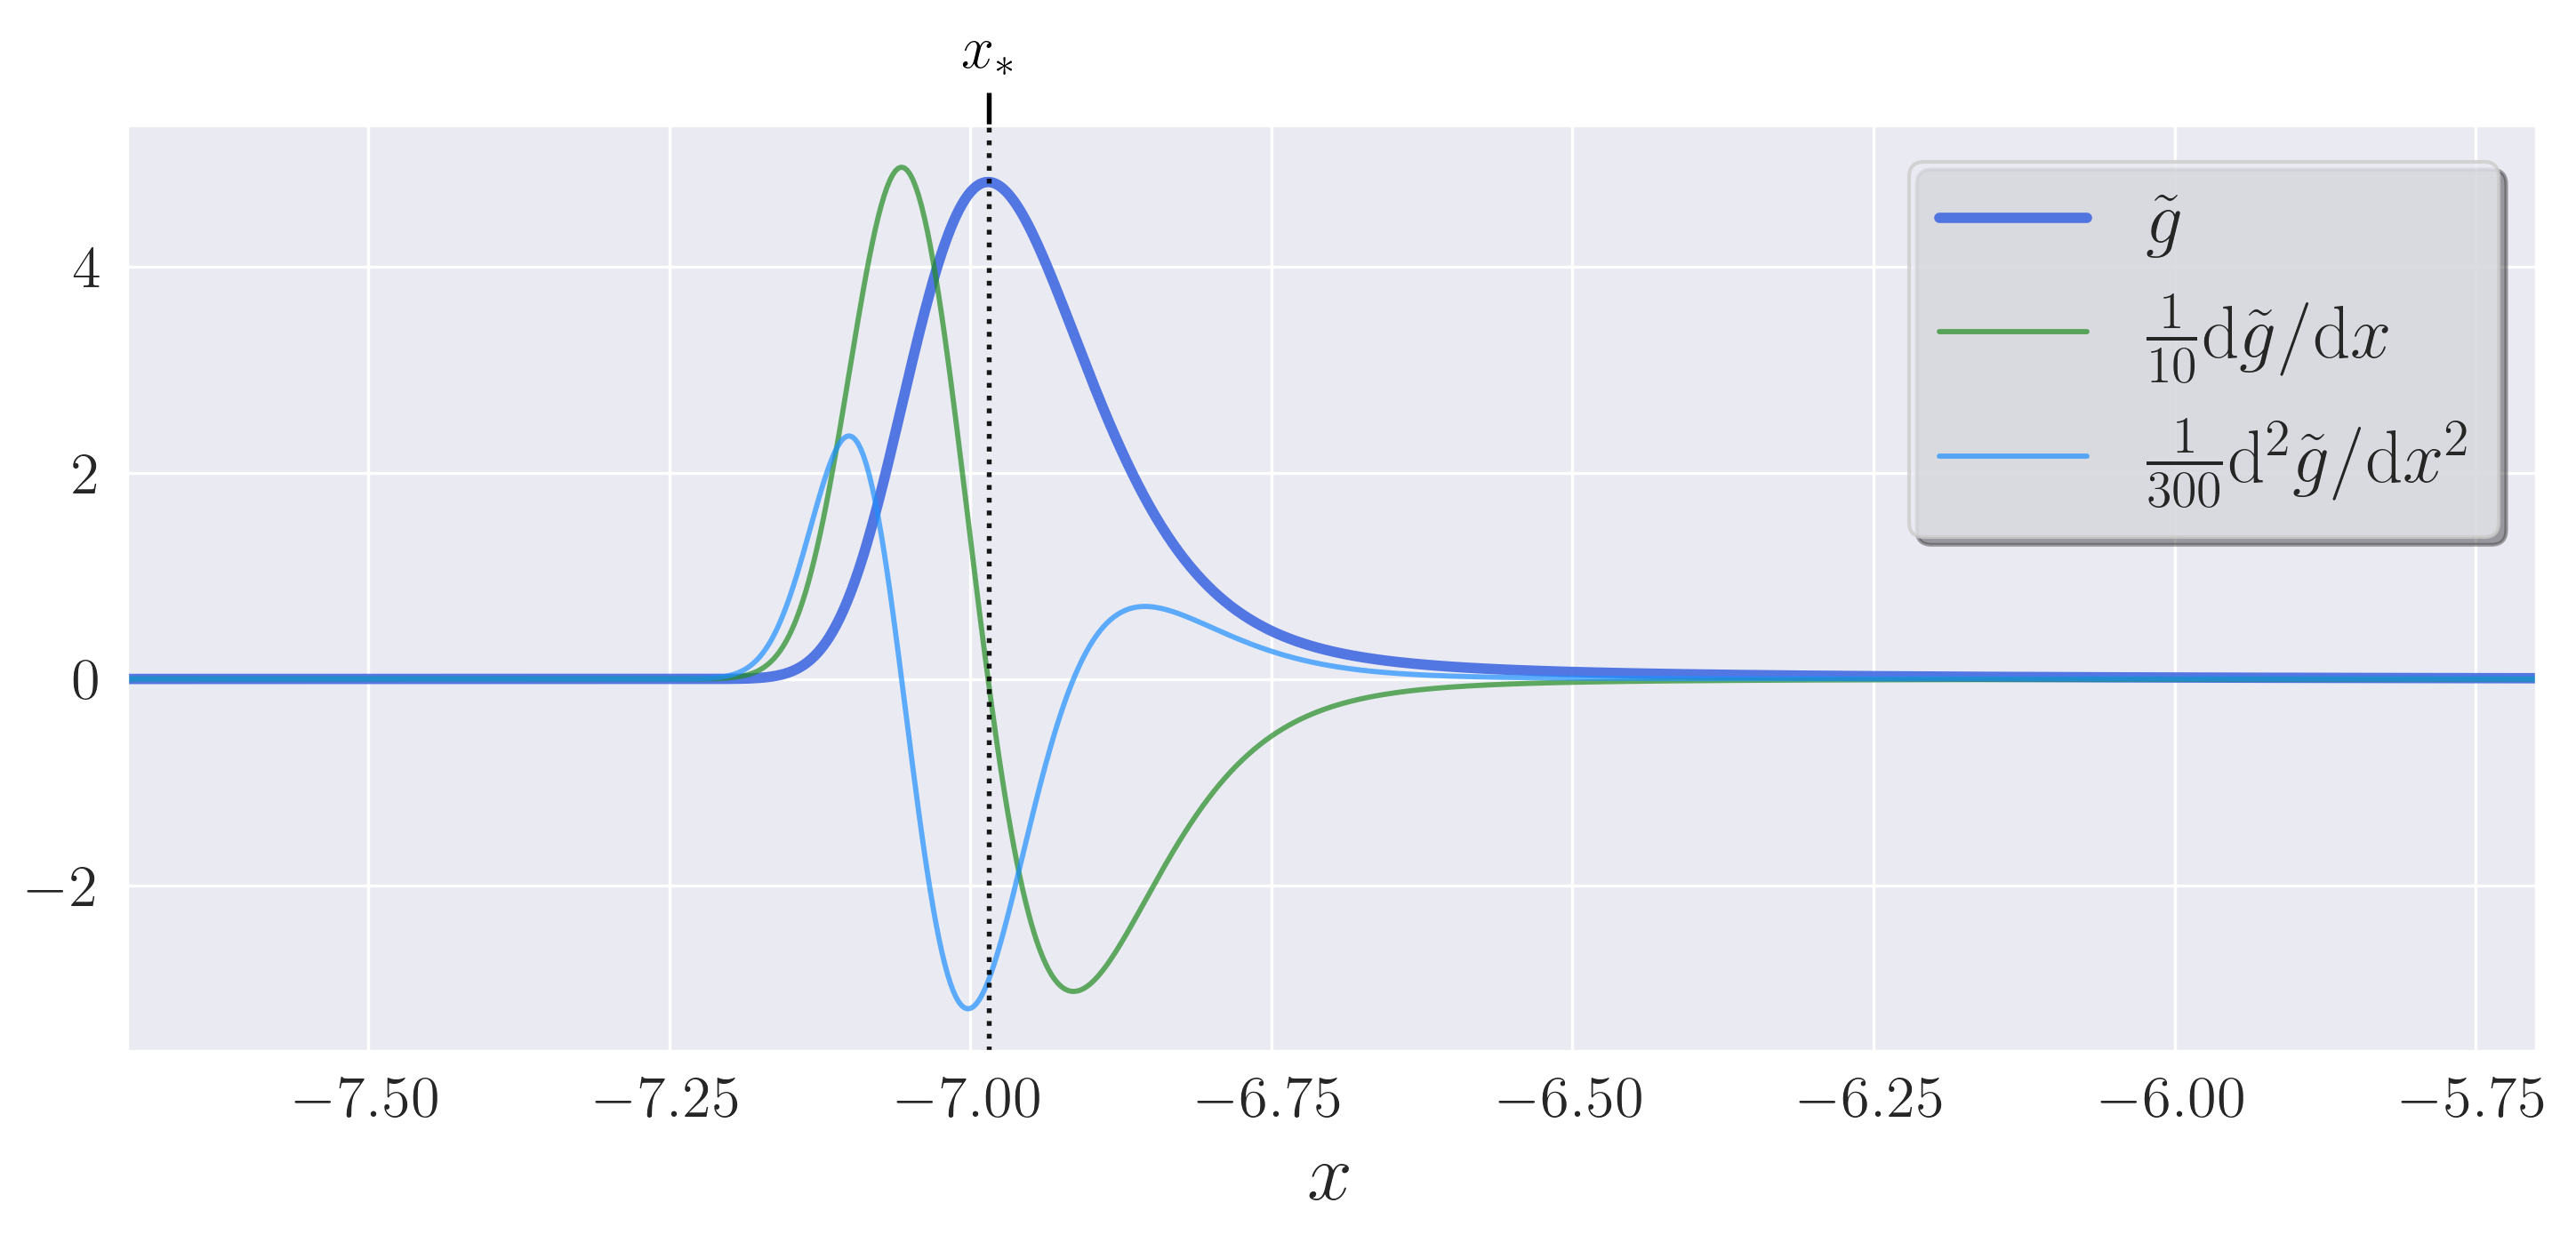
\includegraphics[width=\linewidth]{milestone2/visibility_function_misc.png} 
    \caption{The visibility function $\gt(x)$ and the shape of its derivatives $\dv{\gt(x)}{x}$ and $\dv[2]{\gt(x)}{x}$ as functions of logarithmic scale factor $x$. Recombination onset is shown as the dotted vertical line.} 
    \label[fig]{mil2:res:fig:visibility_function}
\end{figure}

Using the definitions of the time of last scattering surface and recombination presented in~\cref{mil2:theo:sec:optical_depth} and~\cref{mil2:theo:sec:recombination}, we measured the logarithmic scale factor, redshift and cosmic time at these events. We present the results in~\cref{mil2:res:tab:time_of_events} in addition to today's value of the freeze-out electron abundance and the sound horizon at decoupling. The number of significant figures is exaggerated to point out the small differences. The corresponding values resulting from the Saha equation is included in parentheses.
\begin{table}[h]
    \setlength\tabcolsep{0pt}
    \caption{The values of the logarithmic scale factor $x$, the redshift $z$ and the cosmic time $t$ corresponding to two events in the history of the universe. Values in parentheses are those we get with only the Saha equation.}
    \label[tab]{mil2:res:tab:time_of_events}
    \begin{tabular*}{\linewidth}{@{\extracolsep{\fill}} l *{1}{d{2.4}} *{1}{d{4.4}} *{1}{d{2.7}} }
    \toprule
    % & \multicolumn{3}{c}{Time of event} \\
    & \multicolumn{1}{c}{$x$} & \multicolumn{1}{c}{$z$} & \multicolumn{1}{c}{$t$} \\
    \midrule
    Rad.-matter equality  & -8.132 & 3400    & 51.06\unit{ka} \\
    Acceleration onset         & -0.4869 & 0.6272 & 7.752\unit{Ga} \\
    Matter-DE equality    & -0.2558 & 0.2915 & 10.37\unit{Ga} \\
    Today                 & -0.000 & 0.000   & 13.86\unit{Ga} \\
    \midrule
    \multicolumn{2}{l}{Conformal time today:} & \multicolumn{2}{c}{$\eta_0 = 46.32 c$~Ga}\\
    \bottomrule
\end{tabular*}
\end{table}

In the analysis, we used that $x_*=-6.9853$ at the peak of the visibility function.